% Techniques, sensors and frameworks used in autonomous technologies

\chapter{Autonomous Vehicle concepts}
\label{ch:concepts}

In essence, AVs are robots (with 2 degrees of freedom, generally) and more specifically fall in the branch called \textbf{Mobile Robotics}. The following pages will explore the basic concepts of it and what are the tools available to tackle this field.

\section{What is Mobile Robotics}

\subsection{Examples of mobile robotics}

The use of robots to assist or substitute human labour dates back to the 1960s \citeauton{Craig2004} with industrial manipulators and to this day remains as one of the most successful applications of this field. However, generally these robots lack moving capabilities, thus they are limited to a narrow operating environment. 

Mobile Robotics is a relatively recent branch of robotics which aims at developing platforms with moving capabilities \citeauton{Siegwart2004}, in order to achieve tasks that are impossible to do for fixed robots.

Applications in the field of mobile robotics range from:

\begin{itemize}
  \item \textbf{Material delivery}: This is the case for Kiva Systems, company acquired by Amazon in 2012, and whose core idea is to use swarms of mini-robots to transport materials across the warehouse \citeauton{Andrea2012}. Mobile robots (in this case drones) have started to be used by companies like Amazon, Google and DHL to develop last mile delivery logistics \citeauton{Menouar2017a}.

  \item \textbf{Home applications}: This field is where the house cleaning robots called Roomba developed by \href{https://www.irobot.es/}{iRobot} lie. These platforms are equipped with different sensors that allow them to map their environment and navigate in order to clean the rooms of the household \citeauton{Woyke2017}.

  \begin{figure}[t]
    \centering
    \subfloat[Kiva system's robot in a warehouse]{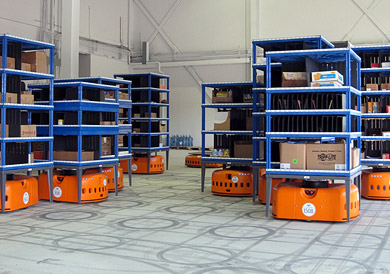
\includegraphics[width=.45\linewidth]{pictures/02/kiva}} \quad
    \subfloat[iRobot's Roomba]{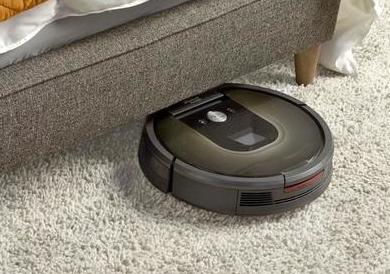
\includegraphics[width=0.45\linewidth]{pictures/02/roomba}}   
    \label{fig:kivarromba}
    \caption[Kiva Systems and Roomba]{Kiva System's robots and Roomba share some design principles}
  \end{figure} 

  \item \textbf{Autonomous Vehicles}: As it was shon on \autoref{ch:intro}, there are many possible areas where self-driving vehicles could be applied.

  \item \textbf{Unknown Environment Exploration}: Robots with moving capabilities are employed to explore unknown environments in rescue missions \citeauton{Bernard2011} or in other planets \citeauton{Grotzinger2013}.
  
  \item \textbf{Defense}: As it has happened with many other scientific advances in history, there is interest in developing mobile robotics with military goals. This is the case of Boston based company \href{https://www.bostondynamics.com/}{Boston Dynamics} and their four-legged robot BigDog \citeauton{Raibert2008} capable of travelling through diverse outdoor terrains.

  \begin{figure}[t]
    \centering
    \subfloat[NASA's Curiosity rover on Mars]{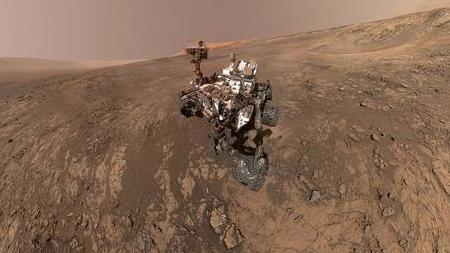
\includegraphics[width=.45\linewidth]{pictures/02/curiosity}} \quad
    \subfloat[Boston Dynamic's SpotMini (2018)]{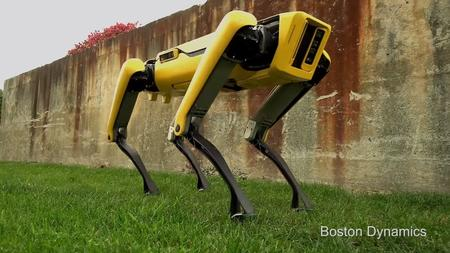
\includegraphics[width=0.45\linewidth]{pictures/02/boston}}   
    \label{fig:curiosityboston}
    \caption[Curiosity and SpotMini robots]{Built to explore the unknown, with different goals in mind}
  \end{figure}
\end{itemize}

\subsection{Robot control paradigms}

The paradigms of control for mobile robotics are very similar to the ones used in robotics and control in general \citeauton{Burgard2017}. Many of the robots mentioned above follow the classical paradigm of sense-plan-act (\autoref{fig:classiccontrol}). The explanation of it is very straightforward: robot senses the environment, then feeds its algorithms with that data and produces an output, that goes into the system's actuators. That response is measured in the next iteration, forming a closed-loop.

\begin{figure}[htb]
  \centering
  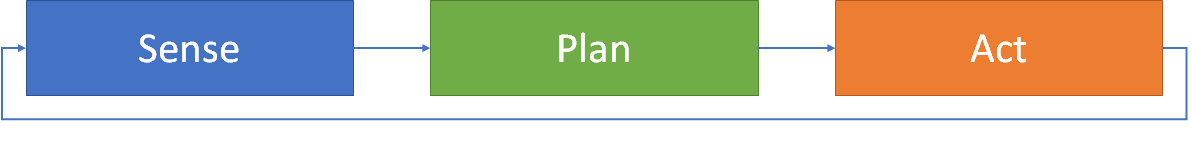
\includegraphics[width=\linewidth]{pictures/02/controlclassic}
  \caption{Classical control paradigm}
  \label{fig:classiccontrol}
\end{figure}

However, this approach requires a larger amount for computing power, which is not suitable for smaller platforms like the Roomba or other home robotics \citeauton{Burgard2017}. Therefore, these types of robots used a more reactive paradigm, where the planning step is removed and substituted by direct mapping of the sensor inputs to specific commands (\autoref{fig:reactive}).

\begin{figure}[htb]
  \centering
  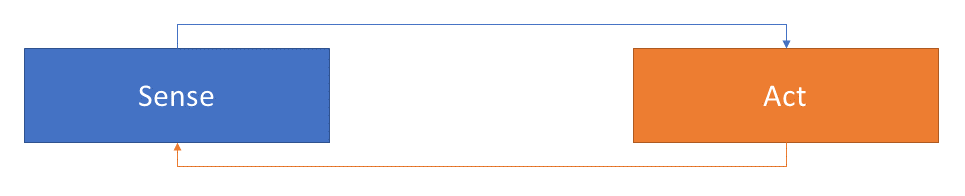
\includegraphics[width=.9\linewidth]{pictures/02/reactive}
  \caption{Reactive control paradigm}
  \label{fig:reactive}
\end{figure}

For the case of self-driving vehicles, the first approach is more suitable, since situations these robots encounter tend to be more complex and require a greater understanding of the environment \citeauton{Siegwart2004}. That is why the classical paradigm is preferred and used in AVs. \autoref{fig:control}, shows a more fine grained description of the control of an autonomous vehicle like the PEV.

\begin{figure}[htb]
  \centering
  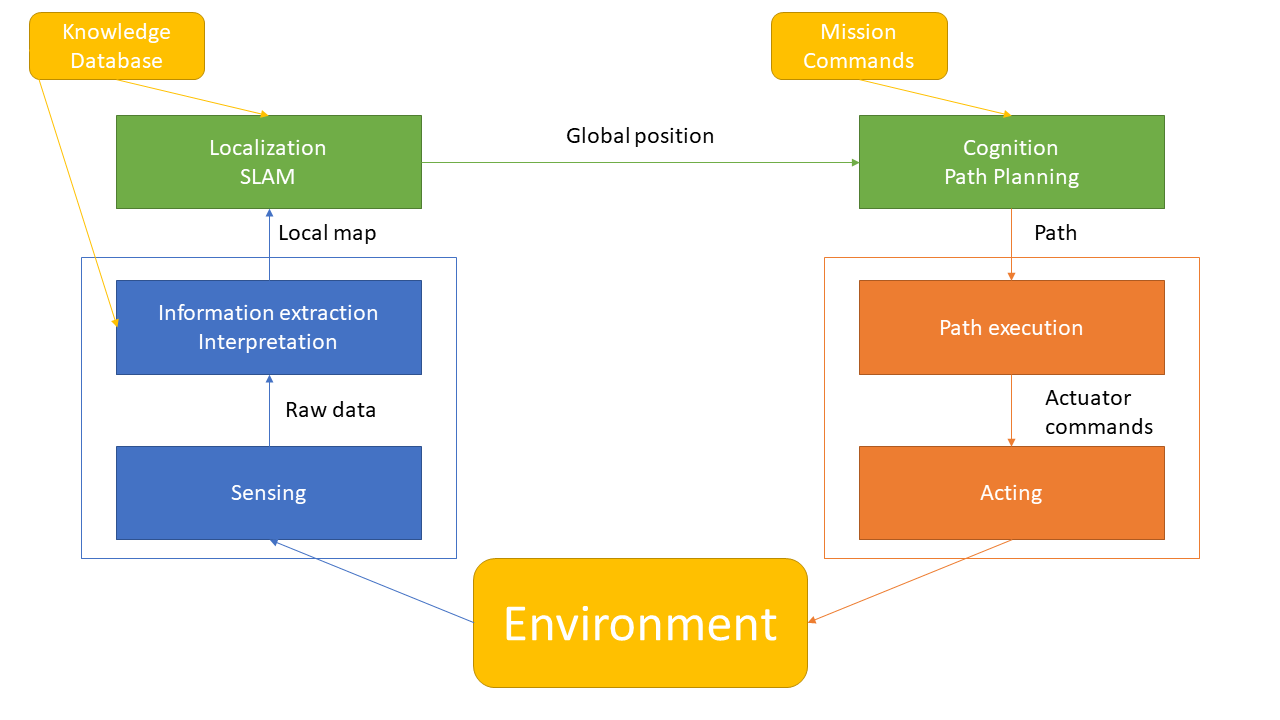
\includegraphics[width=\linewidth]{pictures/02/control}
  \caption{Extended control paradigm for mobile robots}
  \label{fig:control}
\end{figure}

The 3 aspects of control are present (sense-plan-act) but each one is subdivided in different categories. Each one of these constitutes is equally important to consider when building an autonomous platform and they will be described in the following section.

\section{Fundamentals of mobile robotics}

\subsection{Control and Locomotion}

It has been mentioned before that classical robotic arms operate generally fixed to the ground in environments with moving objects, whereas mobile ones are in charge of navigating in mostly static scenarios. Therefore, it can be deduced that mobile robot's most fundamental feature is \textbf{locomotion} \citeauton{Siegwart2004} and it plays an important role on the design of the platform. 

Locomotion can take various forms but the most studied mobile robots are \textbf{legged} and \textbf{wheeled} (\autoref{fig:legwheel}). 

\begin{figure}[htb]
  \centering
  \subfloat[Boston Dynamics' Atlas]{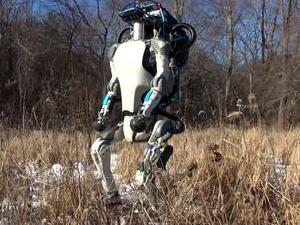
\includegraphics[width=.45\linewidth]{pictures/02/atlas}} \quad
  \subfloat[Yujin Robot's turtlebot]{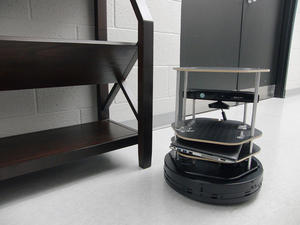
\includegraphics[width=.45\linewidth]{pictures/02/turtlebot}}
  \caption{Legged vs Wheeled robots}
  \label{fig:legwheel}
\end{figure}  

This thesis explores more in detail wheeled locomotion, since it is the basis for both robots that will be described in \autoref{ch:nexus} and \autoref{ch:pev}.

The wheel is by far the most popular mechanism for movement and there are various types \citeauton{Burgard2017a}:

\begin{itemize}
  \item \textbf{Differential drive}: These robots have 2 driving wheels and having each a motor attached. Movement varies due to 'differences' in the speed of both wheels.

  \item \textbf{Car drive (Ackerman steering)}: In this case one motor is in charge of the forward movement, whereas the other one steers the wheels.

  \item \textbf{Omnidirectional drive}: These robots are capable of moving in any direction at any time by using spherical, castor or Swedish wheels (\autoref{fig:omni}).

  \item \textbf{Tracked locomotion}: When driving through loose terrains, wheels are put on a track so that the vehicle gains stability and maneuverability (for example in tanks as shown in \autoref{fig:tank}).

\end{itemize}

\begin{figure}[htb]
  \centering
  \subfloat[Robot with Omnidirectional drive \label{fig:omni}]{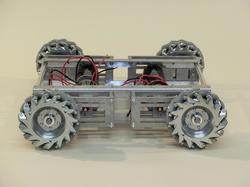
\includegraphics[width=.45\linewidth]{pictures/02/omni}} \quad
  \subfloat[Tanks make use of tracked locomotion \label{fig:tank}]{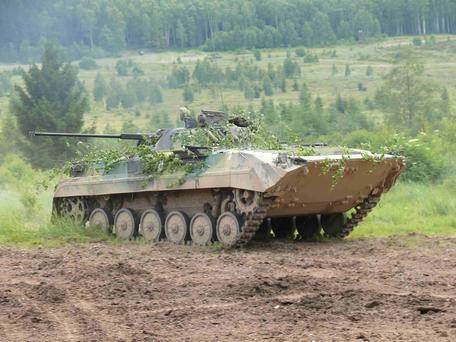
\includegraphics[width=.45\linewidth]{pictures/02/tank}}
  \caption{Omnidirectional and tracked motion examples}
  \label{fig:omnitank}
\end{figure}  

In the next paragraphs, differential drive and ackermann steering will be described in more detail, since those models were used in the Nexus Robot and the PEV respectively.

\parunder{Differential drive} There are many configurations for differential drive robots as it is illustrated in \autoref{fig:diff}. Lets suppose that right and left wheels rotate at velocities $v_r$ and $v_l$ respectively, and that they are separated a distance $L$ (\autoref{fig:diffeq}).

\begin{figure}[htb]
  \centering
  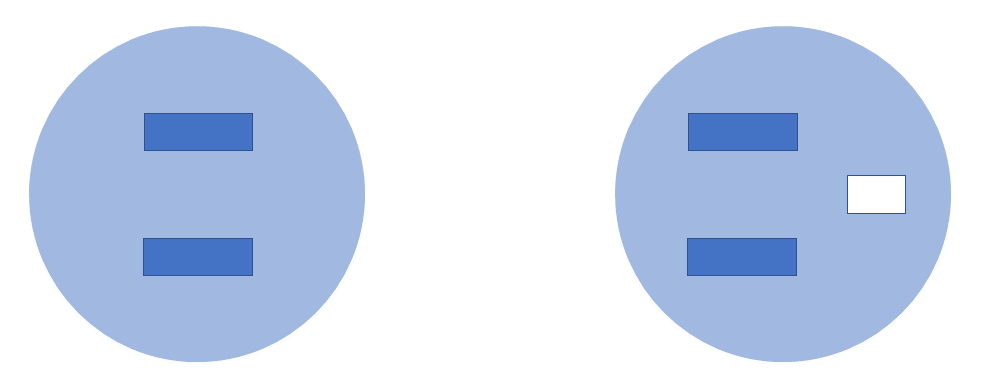
\includegraphics[width=.7\linewidth]{pictures/02/diff}
  \caption[Differential drive modes]{Differential drive modes: 2 motorized wheels (left) or 2 motorized wheels + caster (right)}
  \label{fig:diff}
\end{figure}

\begin{figure}[htb]
  \centering
  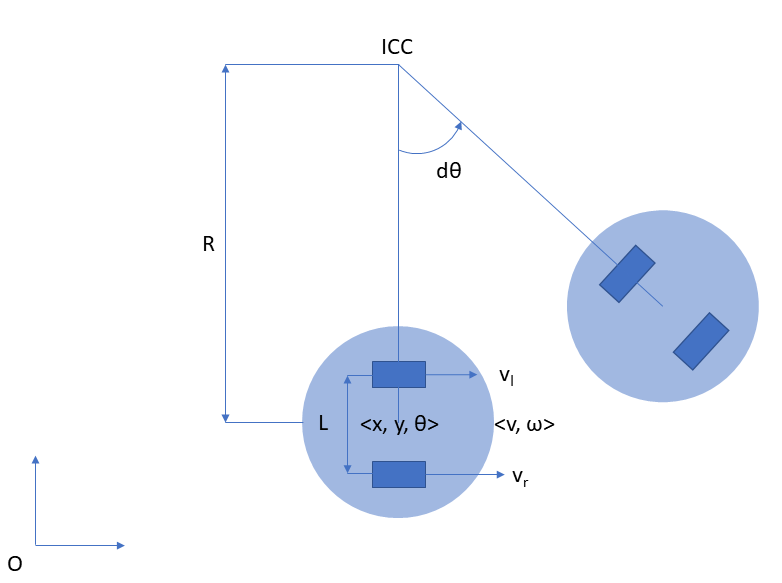
\includegraphics[width=.9\linewidth]{pictures/02/diffeq}
  \caption{Instantaneous movement of a differential drive robot}
  \label{fig:diffeq}
\end{figure}

The movement of the robot is modelled as a rotation at angular speed $\omega$ around the Instantaneous Center of Curvature, ICC (it is shown as $R$ in \autoref{fig:diffeq}).

Both wheel velocities, R and $\omega$ are related through the following equations:
\begin{gather}
  v_l = \omega\cdot(R-\frac{L}{2})\\
  v_r = \omega\cdot(R+\frac{L}{2})
  \label{eq:vrl}
\end{gather} 

From which both $R$ and $\omega$ can be obtained:
\begin{gather}
  R = \frac{L}{2}\cdot\frac{v_r + v_l}{v_r - v_l}\\
  \omega = \frac{v_r - v_l}{L}
  \label{eq:Rw}
\end{gather}  

From these values, the velocity of the robot, $v$ is deduced:
\begin{equation}
  v = \omega \cdot R = \frac{v_r + v_l}{2} 
  \label{eq:v}
\end{equation}

From these equations it can be deduced that differential drive vehicles are able to perform either pure translations (if $v_r$ and $v_l$ are equal) rotate in place (if $v_r$ and $v_l$ are opposite) \citeauton{LaValle2006}.

Both linear and angular velocities are expressed in the local frames, so they are transformed to the base frame:
\begin{gather}
  ^{0}\mathbf{v} = ^{0}\!\!\mathbf{R}_A\cdot^{A}\!\mathbf{v} \label{eq:traf} \\
\begin{bmatrix} \dot{x} \\ \dot{y} \\ \dot{\theta} \end{bmatrix} = 
  \begin{pmatrix} cos\,\theta & -sin\,\theta & 0 \\ sin\,\theta & cos\,\theta & 0 \\ 0 & 0 & 1 \end{pmatrix} \cdot \begin{bmatrix} v \\ 0 \\ \omega \end{bmatrix} = 
  \begin{bmatrix} v\cdot cos\,\theta \\ v\cdot sin\,\theta \\ \omega \end{bmatrix}
    \label{eq:vwtraf}
\end{gather}  

The trajectory is computed by integrating each term over time:
\begin{equation}
  \begin{bmatrix} x \\ y \\ \theta \end{bmatrix} = 
    \begin{bmatrix} \int\limits_0^t v(t) cos(t) dt\\ \int\limits_0^t v(t) sin(t) dt \\ \int\limits_0^t\omega(t)dt \end{bmatrix} = 
    \begin{bmatrix} \frac{1}{2}\!\int\limits_0^t (v_r(t)+v_l(t)) cos(t) dt\\ \frac{1}{2}\!\int\limits_0^t (v_r(t)+v_l(t)) sin(t) dt \\ \frac{1}{L}\!\int\limits_0^t(v_r(t) - v_l(t))dt \end{bmatrix}
\end{equation}  

\parunder{Ackerman steering}

There are various modifications of the Ackerman steering vehicle as well (\autoref{fig:ack}). These vehicles need 2 commands, the drive speed $v$ and the steering angle $\varphi$. Supposing a robot with Ackerman steering whose wheel distance is L, and that the movement can be modelled as a rotation around the ICC (same as differential drive).

\begin{figure}[htb]
  \centering
  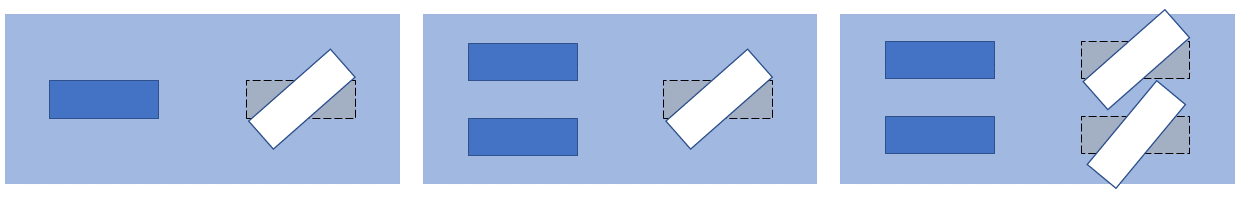
\includegraphics[width=\linewidth]{pictures/02/ack}
  \caption[Ackermann drive modes]{Ackerman drive modes: bicycle (left), tricycle (center), car (right)}
  \label{fig:ack}
\end{figure}

Obtaining the linear speed is trvial (it is s itself), thus only the calculation of the angular speed is needed. Looking at \autoref{fig:ackeq}, it can be seen that:
\begin{gather}
  v = \rho\cdot\omega \\
  \frac{L}{\rho} = tan\,\varphi
\end{gather}  

This yields the result for $\omega$:
\begin{equation}
  \omega = \frac{v}{L}tan\,\varphi
\end{equation} 

The velocities in global coordinates and the translation are computed with the same equations the differential drive robots use. However, there is a fundamental difference between both locomotions: for Ackerman steering robots, it is not possible to rotate in place since that would require the backwheels to slide instead of roll \citeauton{LaValle2006}.

\begin{figure}[htb]
  \centering
  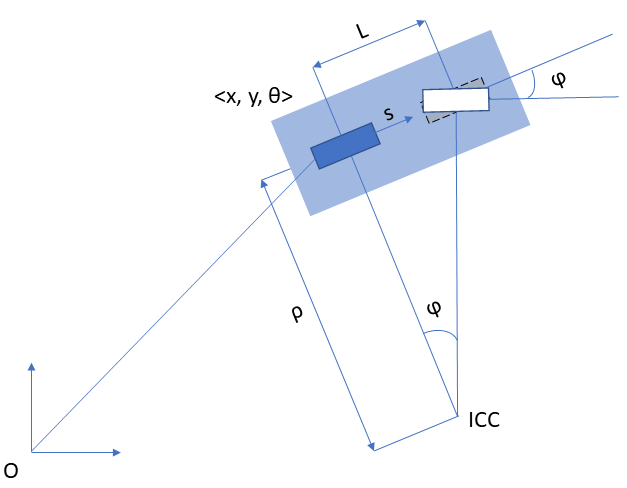
\includegraphics[width=.9\linewidth]{pictures/02/ackeq}
  \caption{Instantaneous movement of an Ackerman drive robot}
  \label{fig:ackeq}
\end{figure}

\subsection{Perception} \label{sub:perception}

Apart from kinematics, acquiring information from the environment is an essential feature, not only of mobile robotics but many other systems \citeauton{Siegwart2004}. \textbf{Sensors} are the ones in charge of that information gathering and they can be divided in \citeauton{Burgard2017b, Burgard2017c}:
\begin{itemize}
  \item \textbf{Active/Passive}: Active sensors emit energy to the environment and measure the response (lasers, radars) and passive sensors measure external inputs (cameras, tactiles).

  \item \textbf{Proprioceptive/Exteroceptive}: Whether the sensor measures internal (speed, joint angles) or external (distance, sound) values.
\end{itemize} 

Sensors can be categorized based on their specific function as well. In the next paragraphs some of these sensors will be described, specially the ones used on the PEV, but there is a wealth of other options that are more suited to other applications \citeauton{Fossen2017, Borenstein1996}.

\parunder{Dead--reckoning and Odometry sensors} Dead--reckoning is the process of determining the current position based on previous state knowledge and the undertaken actions \citeauton{Borenstein1996, Borenstein1997}. One of the most important and widely used implementations of dead--reckoning is \textbf{odometry}, since it is accurate in the short--term, although it drifts over time \citeauton{Borenstein1997}. 

The most used sensors to measure odometry are \textbf{optical encoders}, which consists of a light source passing through a punched disc producing a number of pulses per rotation. Counting the number of pulses (p) in a $\Delta t$, given that the disc has N pulses per revolution can provide the angular velocity:
\begin{equation}
  \omega = \frac{p}{N}\frac{2\pi}{\Delta t}\,\left[\frac{rad}{s}\right]
  \label{eq:odometer}
\end{equation}

If a second channel is added and shifted 90 degrees, rotation direction can be measured as well as position determination becomes more precise (\autoref{fig:encoder}).

\begin{figure}[htb]
  \centering
  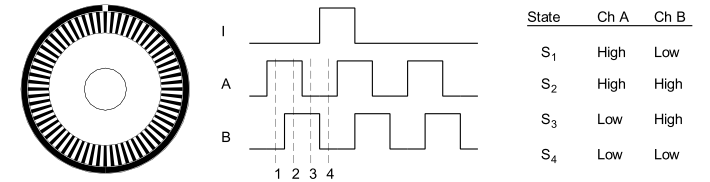
\includegraphics[width=\linewidth]{pictures/02/encoder}
  \caption{Rotary encoder working principle}
  \label{fig:encoder}
\end{figure}  

\parunder{Heading sensors} Heading sensors can help compensate the errors produced in odometry by small differences in orientation \citeauton{Borenstein1996}. This type of sensors are also called \textbf{Inertial sensors} and there are mainly 2 types \citeauton{Borenstein1997}:

\begin{itemize}
  \item \textbf{Accelerometers}: They measure acceleration in one or more axes. However, they perform poorly on many mobile robot applications if used alone.

  \item \textbf{Gyroscopes}: These sensors can measure orientation on 3 axes and are of a notable importance since they correct the odometry measurements when there are small orientation changes.
\end{itemize}  

Recently, another type of sensor has arisen in the field of mobile robotics called \textbf{Inertial Measurment Unit (IMU)}, which combines both accelerometer and gyroscope (sometimes adding a magnetometer for heading).

\parunder{Active/Passive beacons} The principle behind this technology has been used for centuries and it is to determine the absolute position of the robot based on the distance to landmarks or objects whose location is well known \citeauton{Siegwart2004}. This mapping of the position of the robot is done via \textbf{trilateration} or \textbf{triangulation} \citeauton{Borenstein1997}.

Here 2 different systems can be defined: \textbf{Ground--based beacons} and \textbf{Global Positioning System (GPS)}. They vary in that the former uses features or infrastructures located on the ground whereas the latter makes use of a network of satellites specifically built for that purpose (\autoref{fig:gpssch}). 

\begin{figure}[htb]
  \centering
  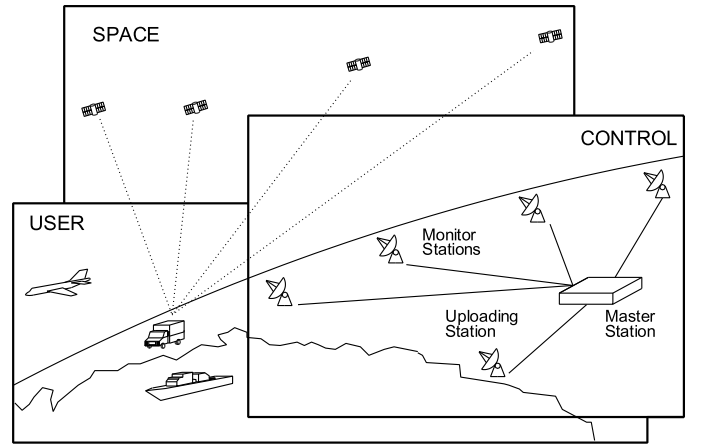
\includegraphics[width=\linewidth]{pictures/02/gps}
  \caption{GPS network overview}
  \label{fig:gpssch}
\end{figure} 

One of the issues these technologie has is that even though it works satisfactorily in outdoor 'open' environments, it is not as suitable in indoor or more 'closed' regions (urban areas with large buildings) \citeauton{Borenstein1996, Borenstein1997}. 

\parunder{Active ranging sensors} This sensors are mostly used for map building and localization. Among all the varieties, the \textbf{Time--of--flight} sensors are the most utilized. These devices send a wave (sound or electromagnetic) and knowing the speed at which they operate, the distance travelled is calculated:
\begin{equation}
  d = \frac{v\cdot t}{2}
  \label{eq:tof}
\end{equation} 

2 types of time-of-flight sensors will be described:
\begin{itemize}
  \item \textbf{Ultrasonic}: This kind of sensor sends a packet pressure waves to determine distance of objects. However, their range goes from 12 cm to 5 m making them unfit for large environments.

  \item \textbf{Laser rangefinders or LIDARs}: It improves the ultrasonic sensor by using infrared light, and it normally adds a rotating mirror so it can cover a wider area. The range of these sensors goes up to 300 m\footnote{https://velodynelidar.com/vls-128.html}. Generally, LiDAR output is a detailed 2D or 3D pointcloud of the surroundings, which often is better than camera+radar based systems. That is why is considered to be the single most important sensor in Autonomous Vehicles \citeauton{Davies2018} and it is also one of the most expensive components.
\end{itemize}  

\parunder{Vision--based sensors} Vision is one of the most powerful senses humans have. It provides with a great deal of information about the surrounding environments and currently there is a lot of effort into building machines with similar capabilities. Recent advances in machine--learning (and deep--learning in particular) \citeauton{LeCun2015}, combined with the existence of many frameworks such as \href{https://www.tensorflow.org/}{Tensorflow} have improved tasks that previously where extremely difficult, such as object detection, scene understanding or lane detection.

The most used vision--based sensors are cameras, among which 2 types can be diferenced:

\begin{itemize}
  \item \textbf{Monocular cameras}: These are well known devices, that have been available in the market for decades.

  \item \textbf{Stereo cameras}: Essentially, the concept is to combine the input images of 2 cameras that watch the scene from different perspectives, and by comparing points that appear on both (conjugate pair), depth information can be obtained (\autoref{fig:zed}).
  \begin{figure}[htb]
    \centering
    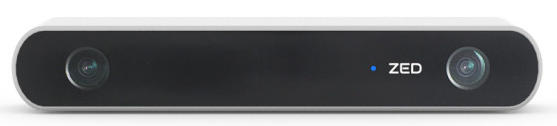
\includegraphics[width=.8\linewidth]{pictures/02/zed}
    \caption{\href{https://www.stereolabs.com/}{ZED} stereo camera}
    \label{fig:zed}
  \end{figure} 
\end{itemize}  

\subsection{Localization} \label{sub:localization}

The problem of localization (which is related to the problem of SLAM that will be discussed in \autoref{ch:slam}) is to determine the position of the robot within the environment \citeauton{Siegwart2004, Thrun2005}.

Recalling the control paradigms in Figures \ref{fig:control} and \ref{fig:reactive}, it is not difficult to see that the former needs a map--based localization system whilst the latter does not. However, the reactive paradigm is not robust to changes in the environment, since it would require to change the rules every time it changed. The classic control one is more scalable beause just by giving the robot another map, it could start navigating in a shorter amount of time.

When a robot is localized it means that the pose of the robot $\mathbf{x_t} = (x\,\, y\,\, \theta)$ is known with respect to the global frame. Nevertheless, pose cannot be sensed, it must be inferred from other sources and sensors are not noise--free, thus making the problem of localization a difficult one \citeauton{Thrun2005}.

\newpage
\parunder{Map representation} The quality of the map is a critical component for a robust localization, therefore much attention has to be paid when choosing a representation \citeauton{Siegwart2004}.

There are mainly 2 manners of representing maps:
\begin{itemize}
  \item \textbf{Continuous representation}: They contain the exact description of their environment. The main advantage is their accuracy at a higher computational cost.
  
  \item \textbf{Decomposed representation}: These type of maps are a higher level abstraction of the area, which results in loss of accuracy but may be useful if the jey features are preserved. One of the most common forms are \textbf{occupancy grid maps}, where the map is discretized an assigned a value if occupied or free.
\end{itemize}  

\parunder{Dimensions of localization} Localization algorithms have a number of divisions \citeauton{Thrun2005}:
\begin{itemize}
  \item \textbf{Global/Local}: In global localization the initial position is unknown, whereas in the local one it is known to be confined in a certain region.

  \item \textbf{Static/Dynamic}: The former are those whose objects remain still and the latter have features that change their position over time.

  \item \textbf{Passive/Active}: In passive localization, the algorithm is limited to observation. In active localization, the algorithm can affect the robot motion to facilitate it.
\end{itemize}  

\parunder{Localization approaches} With regards to the specific algorithms for localization, the main approach is \textbf{probabilistic localization} \citeauton{Thrun2005}. In these branch are included Markov, Extended and Unscented Kalman Filter (EKF and UKF), Grid and MonteCarlo (MCL) localizations. \autoref{fig:locnoloc} shows a working example of a particle filter based localization algorithm, similar to MCL.

\begin{figure}[htb]
  \centering
  \subfloat[Not localized]{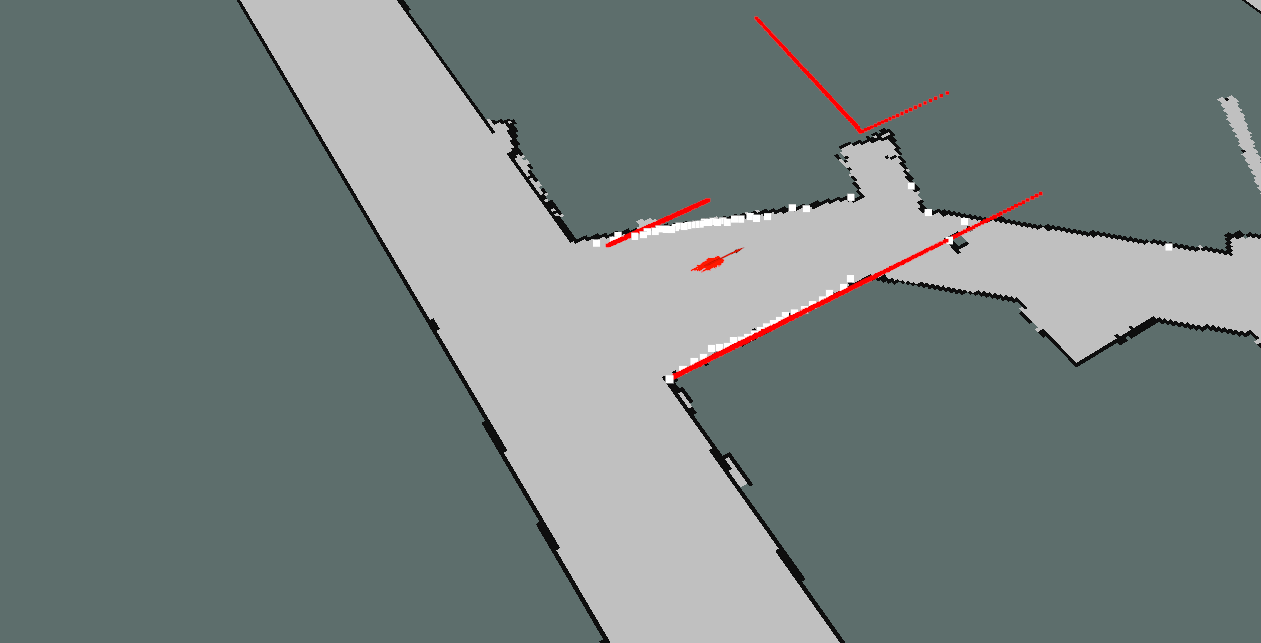
\includegraphics[width=.45\linewidth]{pictures/02/nolocalized}} \quad
  \subfloat[Localized]{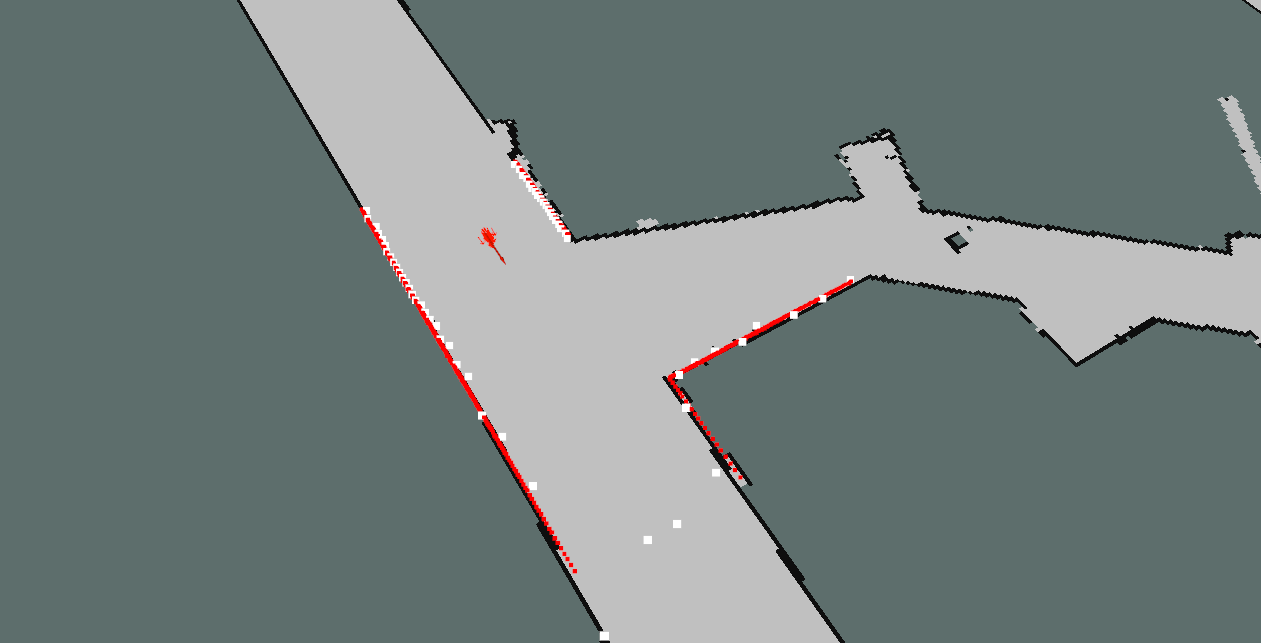
\includegraphics[width=.45\linewidth]{pictures/02/localized}}
  \caption{How probabilistic localization works}
  \label{fig:locnoloc}
\end{figure} 

Those are the most popular algorithms though not unique. Other solutions are landmark--based navigation or route--based navigation. 

\subsection{Planning and Navigation}

Recalling \autoref{fig:control}, it can be inferred that motion planning is the branch that develops algorithms to translate high--level information such maps and human commands into low--level instructions to the controllers \citeauton{LaValle2006}.

Planning and Navigation has 2 goals: reach the desired/commanded location as quickly as possible and avoid obstacles/collisions \citeauton{Burgard2017d}. To achieve that, this task is usually divided in 2 layers as shown in \autoref{fig:plan}.

\begin{figure}[htb]
  \centering
  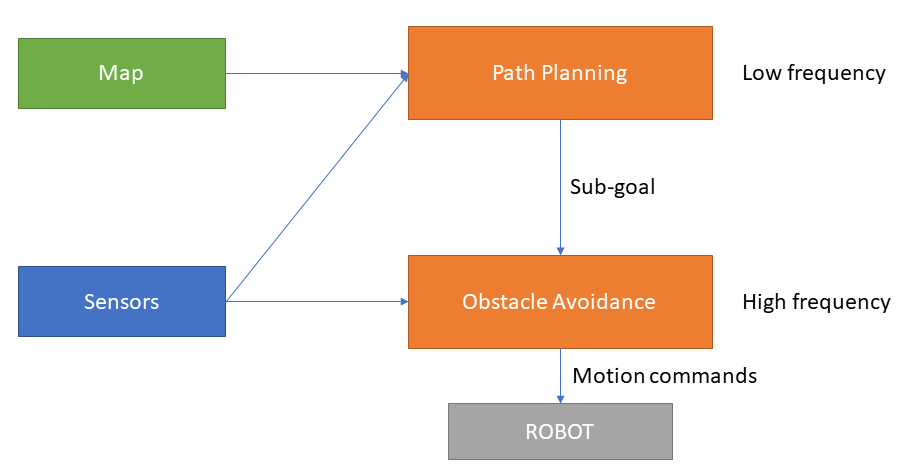
\includegraphics[width=.9\linewidth]{pictures/02/plan}
  \caption{Motion planning workflow}
  \label{fig:plan}
\end{figure} 

\parunder{Path Planning} Path planning can be considered as the long term strategy to reach the goal \citeauton{Siegwart2004}. The objective of this layer is to identify a path that moves to the desired location without hitting any obstacles. For that purpose, the following information is required: The \textbf{start} pose of the robot, the \textbf{goal} pose, the geometrical description of the \textbf{robot} and the representation of the \textbf{environment}. 

The field of path planning was deeply studied for industrial manipulators, and in fact they are more complex cases than differential drive or ackerman steering robots. 

Even though path planning is a real--world problem, when approaching the problem it is often represented in the \textbf{configuration space}, where every state can be represented with k values $q_1, q_2\ldots q_k$, being $k$ the number of degrees of freedom. That space is then discretized and the algorithm is applied. Some of the most common algorithms for path planning are \citeauton{LaValle2006, Burgard2017d}: 
\begin{itemize}
  \item \textbf{Search algorithms}: Such as Dijkstra and A*.

  \item \textbf{Road map planning}: Voronoi diagrams are a very common variety.

  \item \textbf{Cell decomposition}.

  \item \textbf{Rapidly Exploring Random Trees (RRT)}

  \item \textbf{Markov Decision Processes (MDP)}.
\end{itemize}  

\parunder{Obstacle avoidance} Whereas path planning is focused on searching global optimal solutions, obstacle avoidance searches on the local space and modifies the trajectory based on the obstacles detected by sensors. There are many existing algorithms for obstacle avoidance but one of the most utilized (even though there exist more optimal solutions nowadays) is the Dynamic Window Approach (DWA) \citeauton{Fox1997} (\autoref{fig:dwa}).

\begin{figure}[htb]
  \centering
  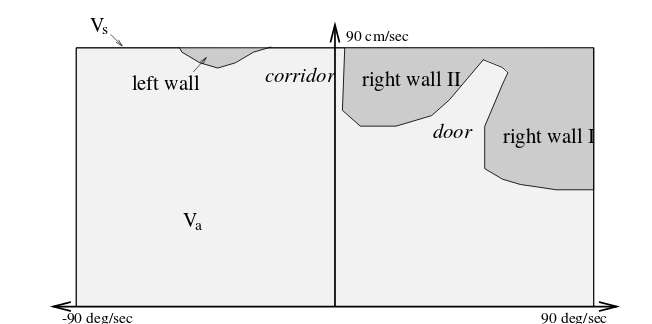
\includegraphics[width=.8\linewidth]{pictures/02/dwa}
  \caption{DWA velocity search space}
  \label{fig:dwa}
\end{figure} 

This algorithm searches the admissible pair of velocities $<v, \omega>$ based on the dynamic constraints and surrounding obstacles that maximize the function:
\begin{equation}
  G(v,\omega)) = \sigma(\alpha\cdot heading(v,\omega)+\beta\cdot dist(v,\omega) + \gamma\cdot vel(v,\omega))
  \label{eq:dwa}
\end{equation}  

where $heading$ measures the distance to the goal (favoring movements towards it), $dist$ the distance to the closest obstacle (favoring clearance) and $vel$ the velocity of the robot (favoring higher speeds).

\section{Robot Operating System (ROS)}

With the rise of robotics, a notable amount of software packages has proliferated these years, either for industrial or research purposes:

\begin{itemize}
  \item \textbf{Industrial robotics software}: Almost every major robot manufacturer ships with their own programming language as it is shown on \autoref{tab:industrial}:

  \begin{table}[htb]
    \centering
    \begin{tabular}{r|l}
      \hline
      \textbf{Company Name} & \textbf{Language Name} \\ \hline
      ABB & \href{https://www.google.com/url?sa=t&rct=j&q=&esrc=s&source=web&cd=1&cad=rja&uact=8&ved=2ahUKEwjFqeGL6e7cAhWHr6QKHS1mBkEQFjAAegQICBAC&url=https%3A%2F%2Flibrary.e.abb.com%2Fpublic%2F688894b98123f87bc1257cc50044e809%2FTechnical%2520reference%2520manual_RAPID_3HAC16581-1_revJ_en.pdf&usg=AOvVaw3zcMHJjAK2YTojeWoqGG_r}{RAPID} \\ \hline
      Kuka & \href{https://drstienecker.com/tech-332/11-the-kuka-robot-programming-language/}{KRL} (Kuka Robot Language) \\ \hline
      Comau & \href{ftp://service.bosso.it/Manuali%20COMAU/IT/handbooks/files/lb-0-0-pdl.pdf}{PDL2} \\ \hline
      Yaskawa & \href{http://spaz.org/~jake/robot/155493-INFORM-LANGUAGE.pdf}{INFORM} \\ \hline
      Fanuc & \href{http://www.onerobotics.com/posts/2013/introduction-to-karel-programming/}{Karel} \\ \hline
    \end{tabular}
    \caption{Industrial robots' programming languages}
    \label{tab:industrial}
  \end{table}

  \item \textbf{Research software}: Some of the libraries used are: Peter Corke's Robotic Toolbox for Matlab \citeauton{Corke}, \href{https://www.microsoft.com/en-us/download/details.aspx?id=29081}{Microsoft Robotics Developer Studio}, \href{https://www.roboticslibrary.org/}{Robotics Library} and many others.
\end{itemize} 

These are not the only items available, in fact the field of robotics is too broad, and there is no perfect solution that covers all the aspects of the it. However, there is one tool that is very popular among researchers and companies around the world and that is called \href{http://www.ros.org/}{Robot Operating System (ROS)}.

\subsection{Why and what is it?}

Every year, robotics grows in size and scaling software becomes a daunting challenge \citeauton{Quigley2009}. This is because robotics gathers the fields of Mechanical and Electrical Engineering with Computer Science, thus software must contain driver level software up to perception and higher levels of abstraction.

Since very few researchers have sufficient knowledge on all the aspects mentioned above, code reuse is a must of any robotics software.

Therefore, in 2008, researchers from Stanford University, University of Southern California (UCSC) and Willow Garage began developing ROS as a continuation of previous software packages such as Stanford's STAIR \citeauton{Quigley2007} and Willow Garage's Personal Robots Program \citeauton{Wyrobek2008}. ROS continued to grow and in 2014, the Open-Source Robotics Foundation (OSRF) took charge of the development and maintenance of the ecosystem\footnote{For more on the history of ROS: \url{http://www.ros.org/history/}}.

ROS was built with the following design goals in mind \citeauton{Quigley2009, Quigley2015} (Figure \autoref{fig:ros} shows a representation of those concepts):

\begin{figure}[htb]
  \centering
  
\includegraphics[width=\linewidth]{pictures/02/ros_equation}
  \caption{Capabilities of ROS}
  \label{fig:ros}
\end{figure}

\begin{itemize}
  \item \textbf{Peer to peer}: ROS consists on different processes that run in a peer--to-peer network exchanging information between them. This way several machines can be attached, performing each one different tasks. For instance, a robot can have several onboard machines sensing and sending actuation commands via ethernet, while offboard machines connected to the previous ones wirelessly can take charge of 'heavier' tasks such as SLAM or Computer Vision (\autoref{fig:peer}).

  \begin{figure}[htb]
    \centering
    % 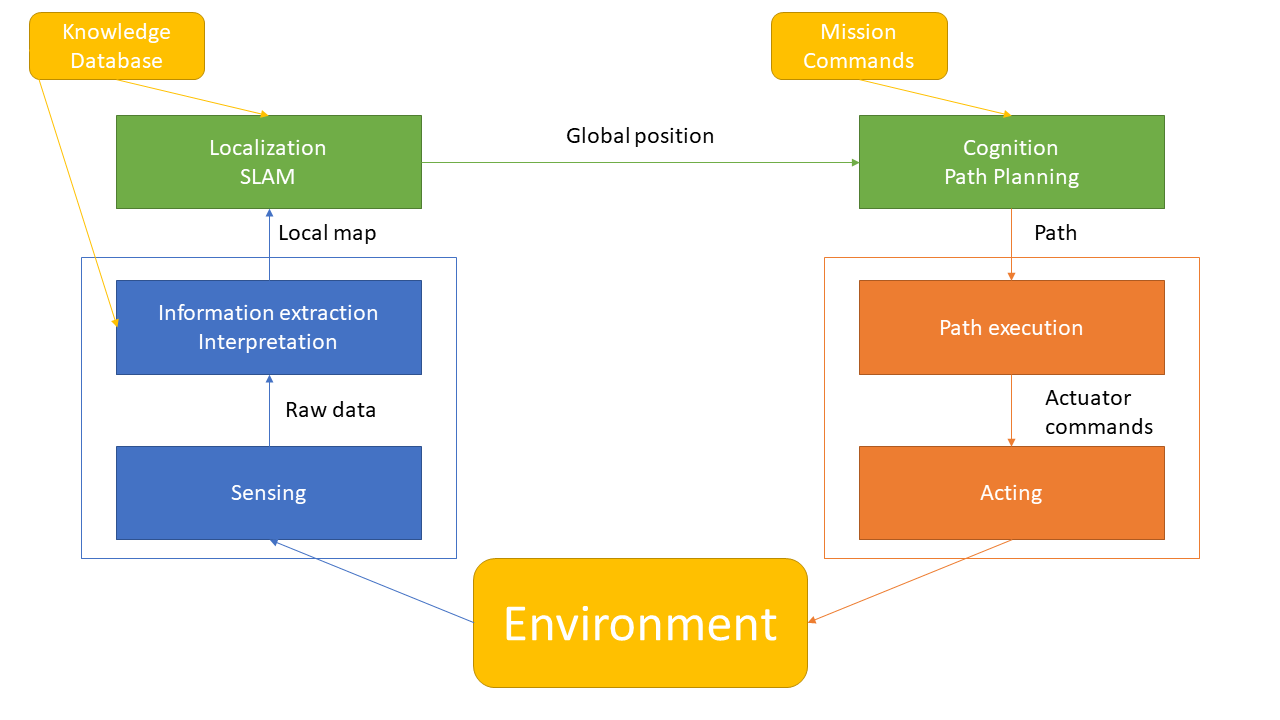
\includegraphics[width=\linewidth]{pictures/02/control}
    \caption{Schematic of the networking capabilities of ROS}
    \label{fig:peer}
  \end{figure}

  \item \textbf{Tools based}: Instead of an enormous standalone application, ROS is composed of several tools with various functionalities, such as navigating the structure, visualizing sensor inputs, compiling, and many others.

  \item \textbf{Multi-lingual}: As every programming language excels at different tasks, ROS provides client libraries for a great variety of languages \footnote{\url{http://wiki.ros.org/Client Libraries}}, being the main ones C++, Python and LISP

  \item \textbf{Thin}: ROS conventions encourage developers to create standalone algorithms and drivers in order to promote code reuse. Those software packages can then be wrapped around ROS and be used on the netowork.

  \item \textbf{Free and Open-Source}: ROS full source is publicly available and anyone can make contributions to its core. This core is licensed under BSD, thus allowing for either commercial or non commercial use.Individual modules or components can have their own licensing.
\end{itemize}

In a more formal definition, ROS is an open-source framework that includes a collection of tools, libraries and conventions to allow for robotic system development \citeauton{Quigley2015}. 

\subsection{Structure of ROS}

\parunder{Basic Concepts} The structure of ROS is composed of \textbf{nodes}, \textbf{messages}, \textbf{topics} and \textbf{services} \citeauton{Quigley2009, OKane2013}:

\begin{itemize}
  \item \textbf{Nodes}: They are the equivalent of software modules and perform one specific computation. When running an application built on ROS, it will very often be composed of several nodes communicating with each other.

  \item \textbf{Messages}: They are data structures that nodes use to communicate. Messages can be composed of basic types or other messages as shown on \autoref{lst:messages}, where a first file \texttt{point.msg} is created to contain 2 variables referring to the position of an object, and the second one \texttt{points.msg} will store a vector of those points:
  \begin{lstlisting}[float=htb,language=Python,frame=htb,caption={Example message files},label=lst:messages] 
    # First file: point.msg
    float32 x
    float32 y 
    # Second file: pointarray.msg
    std_msgs/header header
    point[] points
  \end{lstlisting}

  \item \textbf{Topics}: They act as the containers for the messages. A single node can \textit{publish} messages to a variety of topics, so that other nodes can \textit{subscribe} to one or more of those topics and perform their computations. Topic names must always start with "/" (\ie  "/topic\_name").

  \item \textbf{Services}: Topics can be read/written by any node and sometimes a more bidirectional form of communication is wanted between 2 nodes, in a similar fashion as web services employ request and response documents. That is why services exist (\autoref{lst:services}).
  \begin{lstlisting}[float=htb,language=Python,frame=htb,caption={Example service file},label=lst:services] 
    # File: myService.srv
    # Here goes the request
    int32 x
    int32 y
    ---
    # Here goes the response
    bool success
    int32 multiplication
  \end{lstlisting}
\end{itemize}  

When many nodes and topics are running at the same time, debugging might become difficult. That is why ROS provides a tool called \texttt{rqt\_graph}, in order to visualize all dependencies among processes (\autoref{fig:graph}).
\begin{figure}[htb]
  \centering
  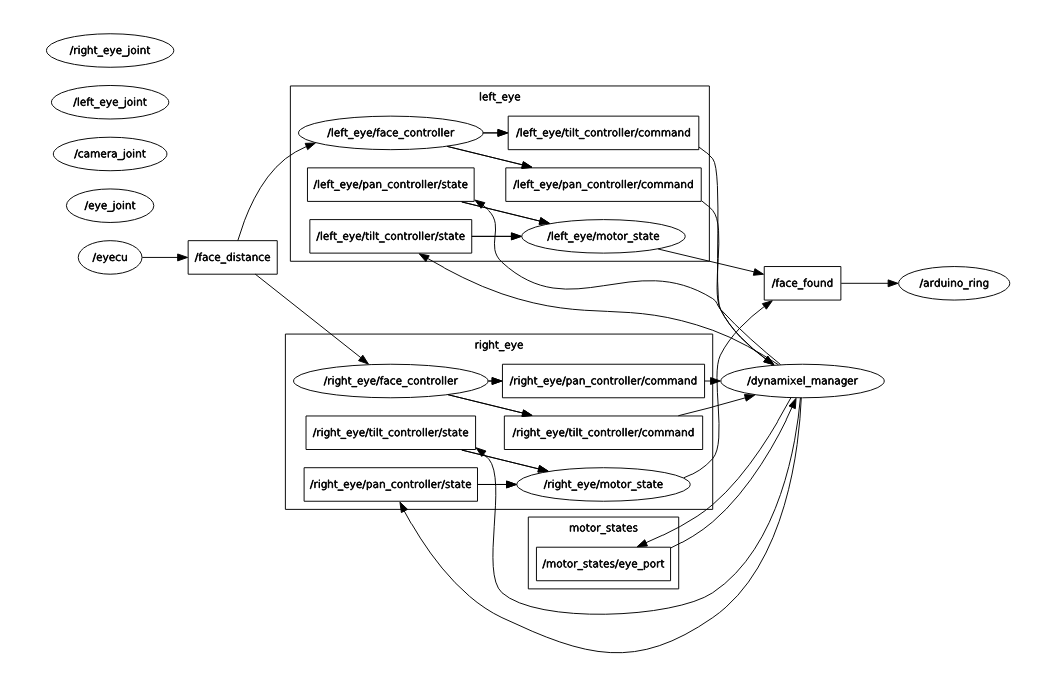
\includegraphics[width=\linewidth]{pictures/02/graph}
  \caption[ROS graph example]{ROS graph example. The flow is represented as: nodes (circles) send messages (arrows) to topics (boxes)}
  \label{fig:graph}
\end{figure}

\parunder{Build system} ROS is packaged with several tools to produce libraries, executables and scripts in both C++ and Python (and other languages with a little tweaking) \citeauton{Quigley2015}. The key concepts here are: \textbf{packages}, \textbf{workspaces} and \textbf{catkin}:

\begin{itemize}
  \item \textbf{Packages}: In ROS, all software, data and documentation is organized into packages. Packages are organized in folders (source code in \texttt{src/}, message files in \texttt{msg/}, launch files in \texttt{launch/}) and need to have 2 files, \texttt{CMakeLists.txt} and \texttt{package.xml} with instructions for the build tools.

  \item \textbf{Workspaces}: Packages are bundled in directories called workspaces, that by convention are called \texttt{exampleworkspace\_ws}. \autoref{fig:ws} shows the structure of workspaces, where packages must be located in the \texttt{src/} folder, and the \texttt{install/} and \texttt{devel/} directories contain the executables and libraries.

  \begin{figure}[htb]
    \centering
    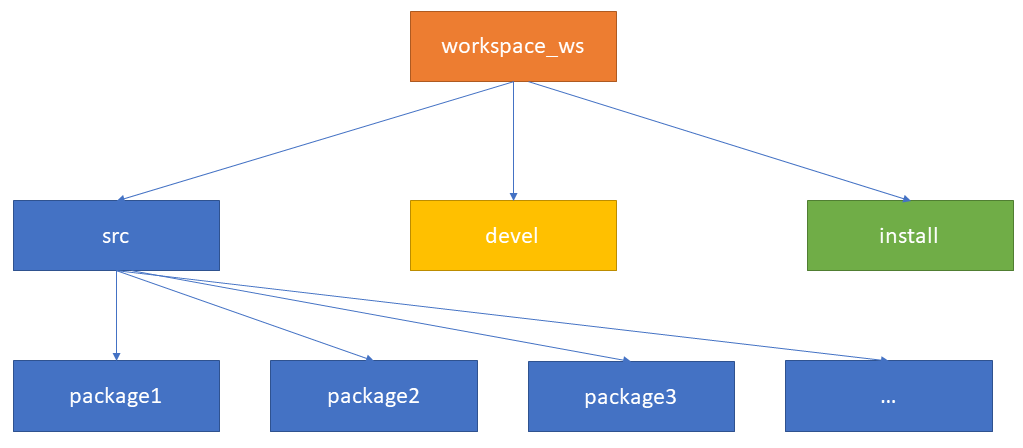
\includegraphics[width=.8\linewidth]{pictures/02/ws}
    \caption{Workspace structure}
    \label{fig:ws}
  \end{figure}

  \item \textbf{Catkin}: It is the offitial build system for ROS. More specifically, it defines some macros and Python scripts to extend the capabilities of CMake, so that building ROS packages is easier \footnote{More information on: \url{http://wiki.ros.org/catkin/conceptual_overview}}. 
\end{itemize}

In order to create the executables, ROS provides the tool \texttt{catkin\_make} and it is used as shown in \autoref{lst:catkin}:
\begin{lstlisting}[float=htb,language=bash,frame=htb,caption={Use of catkin\_make},label=lst:catkin] 
  # Go to workspace
  user@host:~$ cd workspace_ws 
  # Compile packages
  user@host:~/wokspace_ws$ catkin_make 
  # If no errors appear
  user@host:~/wokspace_ws$ source devel/setup.bash
  # This way other ROS tools can find the executables
\end{lstlisting}

\parunder{Running the system} To start any ROS session, there are 3 major components: \textbf{roscore}, \textbf{rosrun} and \textbf{roslaunch}:
\begin{itemize}
  \item \textbf{roscore}: This command launches the ROS master, which is in charge of providing nodes with information to establish communication with other nodes. If the core is not running, nodes cannot find each other and ROS will not start.

  \item \textbf{rosrun}: It searches for the specified node in the specified package and starts it: \texttt{rosrun <package> <executable> <arguments>}.

  \item \textbf{roslaunch}: When the number of nodes and parameters grows in size, it is possible to group several nodes in an \texttt{.xml} file and run them with the \texttt{roslaunch} command (\autoref{lst:roslaunch}). 
  \begin{lstlisting}[float=htb,language=xml,frame=htb,caption={Example of launch file},label=lst:roslaunch] 
    <launch>
    <!-- Node to launch necessary files from Jetson -->

      <!-- Launch hackbike serial -->
      <node pkg="hackbike" type="hackbike_serial" name="hackbike_serial_node" output="screen"/>

      <arg name="mode" default="pedestrian"/>

      <!-- Launch data sender node -->
      <param name="mode" value="$(arg mode)"/>
      <node pkg="panasonic" type="send_data_to_bike.py" name="data_sender_node" output="screen"/>

      <!-- Start tensorflow node -->
      <arg name="tensorflow" default="false"/>
      <group if="$(arg tensorflow)">
        <include file="$(find panasonic)/launch/start_tensorflow.launch"/>
      </group>

      <include file="$(find panasonic)/launch/start_arduino.launch"/>

    </launch>
  \end{lstlisting}
\end{itemize}  

\parunder{Visualization and simulation} It has already been stated that ROS is a tools-based platform, and 2 of those main tools are \textbf{RViz} and \textbf{Gazebo}:

\begin{itemize}
  \item \textbf{RViz}: It is the standard visualization tool for ROS, capable of rendering 3D models, sensed images and pointclouds \citeauton{Gossow2011}. It is widely used for controlling robotic systems based on ROS (\autoref{fig:rviz})
  \begin{figure}[htb]
    \centering
    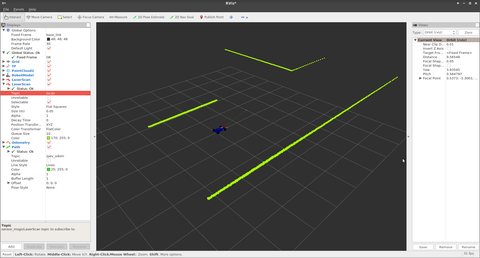
\includegraphics[width=.9\linewidth]{pictures/02/rviz}
    \caption{RViz showing the points received by a LiDAR}
    \label{fig:rviz}
  \end{figure}  

  \item \textbf{Gazebo}: It is an open--source robot simulator with support for multiple robots in complex environments \citeauton{Koenig2004}. It is a different platform from ROS, but they can be bundled together (\autoref{fig:gazebo}).
  \begin{figure}[htb]
    \centering
    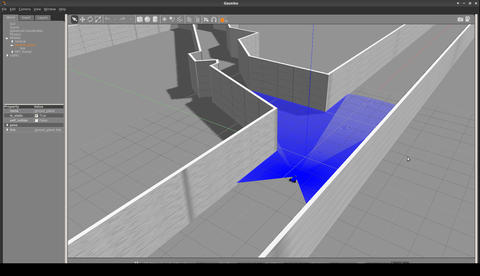
\includegraphics[width=.9\linewidth]{pictures/02/gazebo}
    \caption{Small robot in Gazebo}
    \label{fig:gazebo}
  \end{figure}  
\end{itemize}  

\subsection{Navigation stack}

ROS provides a collection of packages that allow for 2D indoor navigation called Navigation Stack \citeauton{Marder2010}. Basically, this framework reads odometry, laser data and transforms and outputs velocity commands to the controllers. \autoref{fig:navistack} shows a conceptual map of the Navigation Stack. 
\begin{figure}[htb]
  \centering
  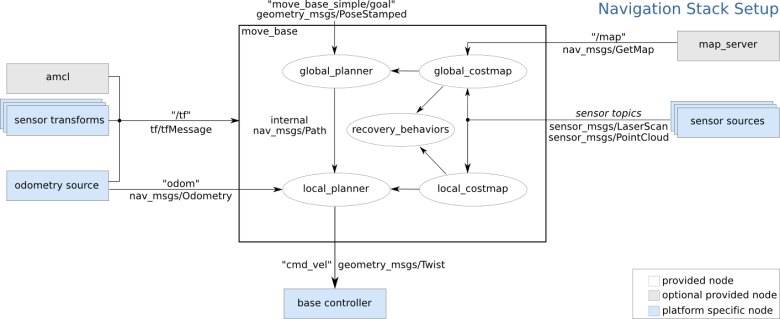
\includegraphics[width=\linewidth]{pictures/02/navistack}
  \caption{Navigation Stack overview}
  \label{fig:navistack}
\end{figure}  

The main nodes provided by the stack are:

\begin{itemize}
  \item \textbf{Global costmap}: It reads the information of a static map and creates a 2D layer with the obstacles detected in it. This layer will remain mostly unchanged. 

  \item \textbf{Local costmap}: It creates a smaller 2D costmap with the available laser data that gets updated frequently in order to account for dynamic obstacles.
  
  \item \textbf{Global planner}: With the information from the global costmap and a desired goal, it provides a high-level plan for the robot to follow. It uses algorithms like Dijkstra or A* and it does not take into account any kinematic or dynamic restrictions.

  \item \textbf{Local planner}: It reads the global plan and the local costmap and outputs velocity commands that follow the global plan as closely as possible while avoiding obstacles. This planner takes into account the constraints the robot might have.
\end{itemize}  

The navigation stack is a useful tool but has its limitations as well. First, it is optimized for 2D navigation which is less accurate and not particularly suitable for large environments. Second, it was designed for indoor navigation not for outdoor scenarios. And third, it only considers differential and holonomic drive robots.

However, it is possible to modify some of the nodes provided to extend the functionalities of the stack, as it has been done with the PEV.
